% --- Contenuto LaTeX autogenerato da capitolo3.md (sezione 4) ---

\section{INTRODUZIONE E ARCHITETTURA GENERALE}

Prima di analizzare nel dettaglio i singoli componenti dell'architettura di Gamma, è fondamentale comprendere la filosofia progettuale e il flusso di elaborazione che governa l'intero sistema. Gamma è concepito come una \textbf{pipeline di trasformazioni successive}, dove ogni livello di astrazione traduce rappresentazioni sempre più concrete fino al risultato sonoro finale.

\subsection{Visione d'insieme del sistema}

Il sistema Gamma implementa una \textbf{separazione netta tra tre domini fondamentali}: la concezione compositiva, l'elaborazione algoritmica e la sintesi sonora. Questa separazione non è meramente tecnica, ma riflette una precisa filosofia compositiva che distingue tra \emph{intenzione}, \emph{interpretazione} e \emph{realizzazione}.

\begin{figure}[htbp]
\centering
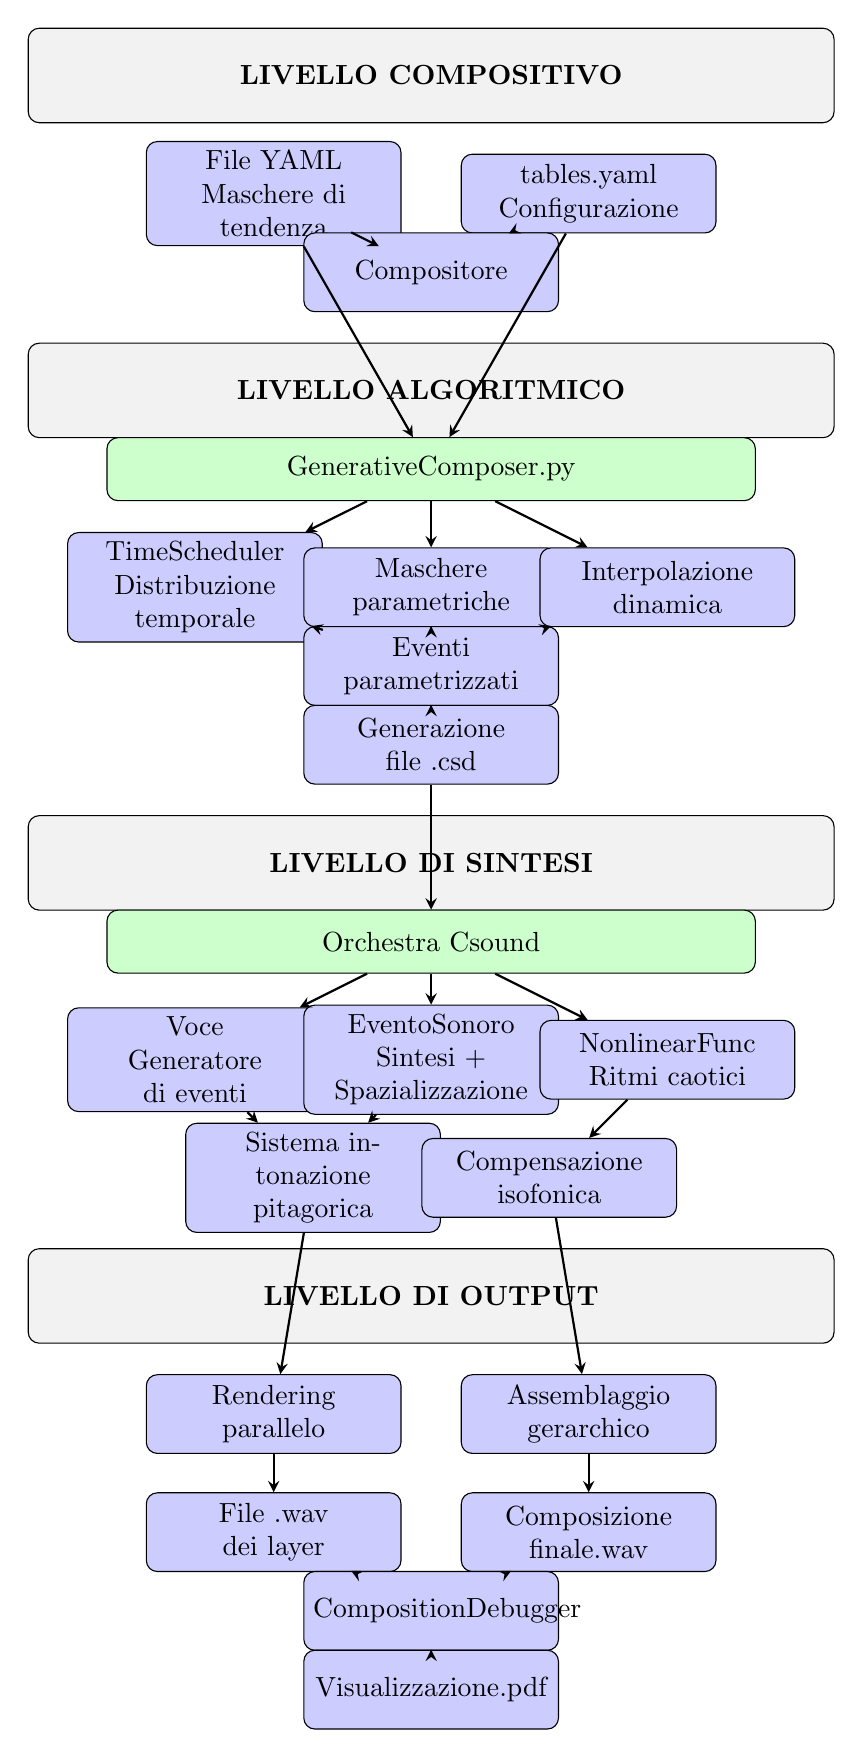
\begin{tikzpicture}[
    block/.style={rectangle, draw, fill=blue!20, text width=3cm, text centered, rounded corners, minimum height=1cm},
    wideblock/.style={rectangle, draw, fill=green!20, text width=8cm, text centered, rounded corners, minimum height=0.8cm},
    levelblock/.style={rectangle, draw, fill=gray!10, text width=10cm, text centered, rounded corners, minimum height=1.2cm, font=\bfseries},
    arrow/.style={thick,->,>=stealth}
]

% Livello Compositivo
\node[levelblock] (comp) at (0,8) {LIVELLO COMPOSITIVO};
\node[block] (yaml) at (-2,6.5) {File YAML\\Maschere di tendenza};
\node[block] (tables) at (2,6.5) {tables.yaml\\Configurazione};
\node[block] (compositore) at (0,5.5) {Compositore};

% Livello Algoritmico  
\node[levelblock] (algo) at (0,4) {LIVELLO ALGORITMICO};
\node[wideblock] (gencomp) at (0,3) {GenerativeComposer.py};
\node[block] (scheduler) at (-3,1.5) {TimeScheduler\\Distribuzione\\temporale};
\node[block] (maschere) at (0,1.5) {Maschere\\parametriche};
\node[block] (interp) at (3,1.5) {Interpolazione\\dinamica};
\node[block] (eventi) at (0,0.5) {Eventi parametrizzati};
\node[block] (csd) at (0,-0.5) {Generazione file .csd};

% Livello di Sintesi
\node[levelblock] (sintesi) at (0,-2) {LIVELLO DI SINTESI};
\node[wideblock] (csound) at (0,-3) {Orchestra Csound};
\node[block] (voce) at (-3,-4.5) {Voce\\Generatore\\di eventi};
\node[block] (evento) at (0,-4.5) {EventoSonoro\\Sintesi +\\Spazializzazione};
\node[block] (nonlinear) at (3,-4.5) {NonlinearFunc\\Ritmi caotici};
\node[block] (pitag) at (-1.5,-6) {Sistema intonazione\\pitagorica};
\node[block] (iso) at (1.5,-6) {Compensazione\\isofonica};

% Livello di Output
\node[levelblock] (output) at (0,-7.5) {LIVELLO DI OUTPUT};
\node[block] (rendering) at (-2,-9) {Rendering\\parallelo};
\node[block] (assemb) at (2,-9) {Assemblaggio\\gerarchico};
\node[block] (layerwav) at (-2,-10.5) {File .wav\\dei layer};
\node[block] (finalwav) at (2,-10.5) {Composizione\\finale.wav};
\node[block] (debug) at (0,-11.5) {CompositionDebugger};
\node[block] (pdf) at (0,-12.5) {Visualizzazione.pdf};

% Frecce
\draw[arrow] (compositore) -- (yaml);
\draw[arrow] (compositore) -- (tables);
\draw[arrow] (yaml) -- (gencomp);
\draw[arrow] (tables) -- (gencomp);
\draw[arrow] (gencomp) -- (scheduler);
\draw[arrow] (gencomp) -- (maschere);
\draw[arrow] (gencomp) -- (interp);
\draw[arrow] (scheduler) -- (eventi);
\draw[arrow] (maschere) -- (eventi);
\draw[arrow] (interp) -- (eventi);
\draw[arrow] (eventi) -- (csd);
\draw[arrow] (csd) -- (csound);
\draw[arrow] (csound) -- (voce);
\draw[arrow] (csound) -- (evento);
\draw[arrow] (csound) -- (nonlinear);
\draw[arrow] (voce) -- (pitag);
\draw[arrow] (evento) -- (pitag);
\draw[arrow] (nonlinear) -- (iso);
\draw[arrow] (pitag) -- (rendering);
\draw[arrow] (iso) -- (assemb);
\draw[arrow] (rendering) -- (layerwav);
\draw[arrow] (assemb) -- (finalwav);
\draw[arrow] (layerwav) -- (debug);
\draw[arrow] (finalwav) -- (debug);
\draw[arrow] (debug) -- (pdf);

\end{tikzpicture}
\caption{Architettura completa del sistema Gamma: flusso di elaborazione dai concetti compositivi al risultato sonoro finale}
\label{fig:gamma_architecture}
\end{figure}

\subsection{Flusso di elaborazione top-down}

Il processo compositivo in Gamma segue un \textbf{approccio a cascata guidato dalle maschere di tendenza}, dove ogni fase raffina e concretizza le informazioni del livello superiore:

\subsubsection{Fase 1: Definizione delle Intenzioni Compositive}
Il compositore opera al livello più astratto, definendo \textbf{spazi di possibilità} piuttosto che valori deterministici. Una maschera come \texttt{ottava: \{ range: [3, 6] \}} non specifica un'altezza precisa, ma delimita una regione tonale che il sistema esplorerà stocasticamente. Questa filosofia si estende a tutti i parametri: dinamiche, durate, densità, comportamenti ritmici.

\subsubsection{Fase 2: Interpretazione e Generazione Parametrica}
Il \texttt{GenerativeComposer} funge da \textbf{interprete delle intenzioni compositive}, traducendo le maschere astratte in parametri numerici concreti per ogni singolo evento sonoro. Questo processo non è meccanico: il sistema implementa strategie di generazione differenziate (distribuzioni gaussiane, scelte pesate, interpolazioni) e gestisce l'evoluzione temporale attraverso l'interpolazione tra stati iniziali e finali.

Il \texttt{TimeScheduler} opera in parallelo, traducendo modelli temporali astratti (\texttt{ritardando}, \texttt{accelerando}, \texttt{breakpoint}) in sequenze precise di onset temporali. Questa separazione tra generazione parametrica e distribuzione temporale permette di orchestrare indipendentemente il \emph{cosa} suona e il \emph{quando} suona.

\subsubsection{Fase 3: Traduzione in Linguaggio Csound}
La generazione degli score \texttt{.csd} rappresenta il \textbf{ponte tra l'astrazione algoritmica e la concretezza della sintesi}. Ogni evento generato viene tradotto in una chiamata allo strumento \texttt{Voce}, che riceve non solo i parametri musicali ma anche metadati strutturali necessari per la gestione dei confini temporali e la coerenza dell'assemblaggio finale.

\subsubsection{Fase 4: Sintesi e Spazializzazione}
L'orchestra Csound implementa una \textbf{gerarchia di responsabilità}: lo strumento \texttt{Voce} gestisce la macro-temporalità e la generazione di sequenze di eventi, delegando a \texttt{EventoSonoro} la sintesi del singolo suono e la sua spazializzazione. Il sistema di intonazione pitagorica e la compensazione isofonica operano trasversalmente, garantendo coerenza armonica e percettiva.

\subsubsection{Fase 5: Assemblaggio e Finalizzazione}
Il rendering finale adotta una \textbf{strategia gerarchica}: prima i layer vengono renderizzati individualmente, poi assemblati a livello di sezione, infine combinati nella composizione completa. Questa architettura permette rendering incrementali e ottimizzazioni per il flusso di lavoro compositivo iterativo.

\subsection{Principi architetturali fondamentali}

L'architettura di Gamma si fonda su tre principi progettuali che ne determinano sia le capacità espressive che le caratteristiche tecniche:

\textbf{Disaccoppiamento modulare}: Ogni componente ha responsabilità ben definite e comunica attraverso interfacce standardizzate. Il \texttt{TimeScheduler} non conosce i contenuti musicali, il generatore parametrico non gestisce la sintesi, l'orchestra Csound non influenza la logica compositiva.

\textbf{Configurabilità esterna}: La separazione tra codice e dati musicali permette modifiche profonde del comportamento senza interventi sul software. Il file \texttt{tables.yaml} estende questo principio anche agli aspetti più tecnici come gli inviluppi e le forme d'onda.

\textbf{Scalabilità computazionale}: L'approccio a rendering parallelo e assemblaggio gerarchico rende il sistema adatto a composizioni di dimensioni arbitrarie, mantenendo tempi di elaborazione gestibili anche per progetti complessi.

Questi principi non sono solo scelte tecniche, ma riflettono una \textbf{visione compositiva} che privilegia l'esplorazione controllata dello spazio sonoro rispetto alla determinazione esatta di ogni dettaglio, permettendo al compositore di lavorare con il sistema come con uno strumento espressivo piuttosto che come con un semplice esecutore di istruzioni.


Il \texttt{generative\_composerYaml2.py} è un sistema di composizione algoritmica che traduce una descrizione astratta di una struttura musicale, definita in formato YAML, in un file audio (WAV). Lo fa generando uno score per il software di sintesi sonora Csound.

L'architettura del programma è basata su tre componenti principali e un'esecuzione a fasi:

\begin{enumerate}
    \item \textbf{\texttt{GenerativeComposer}}: La classe principale che contiene la logica per interpretare la partitura YAML, generare i parametri stocastici degli eventi sonori e creare i file di score \texttt{.csd} per Csound.
    \item \textbf{\texttt{CompositionDebugger}}: Una classe di utilità dedicata esclusivamente alla creazione di una visualizzazione grafica (in formato PDF) della composizione generata, simile a un \textit{piano roll} arricchito con informazioni sulle tendenze parametriche.
    \item \textbf{\texttt{TimeScheduler}}: Una classe specializzata nella generazione di sequenze temporali (gli *onset*, o istanti di inizio) degli eventi, secondo diversi modelli (lineare, accelerando, ritardando, etc.).
\end{enumerate}
Il processo, orchestrato nel blocco \texttt{if \_\_name\_\_ == "\_\_main\_\_":}, non è monolitico ma suddiviso in fasi distinte e sequenziali, che permettono di separare la generazione, il rendering e la visualizzazione.
\subsection{Fase di Input: Caricamento della Struttura della Composizione}
Il punto di partenza è un file YAML. Il programma supporta la definizione di composizioni complesse, articolate in più parti, utilizzando la sintassi multi-documento di YAML (documenti separati da \texttt{{-}{-}{-}}).

La funzione \texttt{load\_all\_compositions\_from\_yaml} si occupa di questo compito:

\begin{lstlisting}[language=Python]
def load_all_compositions_from_yaml(file_path):
    """
    Carica una o più composizioni da un singolo file YAML.
    I documenti multipli devono essere separati da '---'.
    Restituisce una lista di strutture di composizione.
    """
    print(f"Caricamento partiture dal file multi-documento: {file_path}")
    composizioni = []
    try:
        with open(file_path, 'r') as f:
            docs = list(yaml.safe_load_all(f))
        for i, composition in enumerate(docs):
            if composition is None: continue 
            composizioni.append(composition)
        return composizioni
\end{lstlisting}

Ogni documento YAML caricato rappresenta una \textit{Parte} della composizione. Ogni parte è una lista di \textit{Sezioni}, e ogni sezione può contenere uno o più \textit{Layer}. Questa struttura gerarchica (Parte -> Sezione -> Layer -> Evento) è il modello concettuale su cui si basa tutta la logica successiva.

In aggiunta, viene caricato un file \texttt{tables.yaml} che definisce le caratteristiche degli inviluppi (es. attacco, rilascio) che verranno usati da Csound.
\subsection{Il Nucleo Generativo: Dal Concetto ai Parametri}
Il cuore del sistema risiede nella classe \texttt{GenerativeComposer} e nella sua capacità di trasformare le \textit{maschere} parametriche definite nel YAML in valori numerici concreti per ogni evento sonoro.

La generazione avviene all'interno di un \textit{layer}. Un layer può essere:
\begin{itemize}
 \item \textbf{Statico}: Definito da uno \texttt{stato\_unico}. Tutti gli eventi generati in questo layer attingeranno da un'unica maschera di parametri.
 \item \textbf{Dinamico}: Definito da uno \texttt{stato\_iniziale} e uno \texttt{stato\_finale}. I parametri degli eventi evolvono nel tempo, interpolando tra queste due maschere.
\end{itemize}

La funzione \texttt{\_process\_layer} gestisce un singolo layer. I suoi passaggi chiave sono:
\begin{enumerate}
    \item \textbf{Calcolo del Timing}: Determina la durata effettiva del layer basandosi sul \texttt{lifespan} (una finestra temporale relativa alla sezione, es. \texttt{[0.0, 0.5]} per la prima metà).
    \item \textbf{Generazione degli Onset}: Utilizza \texttt{TimeScheduler} per calcolare gli istanti di attivazione dei cluster di eventi all'interno della durata del layer.
    \item \textbf{Generazione degli Eventi}: Per ogni onset, determina la maschera parametrica (statica o interpolata) e genera un \textit{cluster} di eventi sonori.
\end{enumerate}
\subsubsection{Generazione Stocastica dei Parametri (\texttt{\_generate\_params\_from\_mask})}
Questa funzione è il motore stocastico. Prende una \textit{maschera} (un dizionario che descrive un parametro) e produce un valore numerico. Supporta diversi tipi di generazione:

\begin{itemize}
 \item \textbf{Distribuzione Uniforme}: Se la maschera contiene una chiave \texttt{range}.
\end{itemize}

\begin{lstlisting}[language=Python]
elif 'range' in p_mask:
    min_val, max_val = p_mask['range']
\section{...}
    val = random.uniform(min_val, max_val)
\end{lstlisting}
\begin{itemize}
 \item \textbf{Distribuzione Normale}: Se la maschera contiene \texttt{mean} e \texttt{std}.
\end{itemize}

\begin{lstlisting}[language=Python]
if 'mean' in p_mask and 'std' in p_mask:
    mean = p_mask['mean']
    std = p_mask['std']
    val = np.random.normal(loc=mean, scale=std)
\end{lstlisting}
\begin{itemize}
 \item \textbf{Scelta Pesata}: Se la maschera contiene \texttt{choices} ed opzionalmente \texttt{weights}.
\end{itemize}

\begin{lstlisting}[language=Python]
elif 'choices' in p_mask:
    val = random.choices(p_mask['choices'], weights=p_mask.get('weights'), k=1)[0]
\end{lstlisting}

Questa logica viene applicata a tutti i parametri (altezza, durata, etc.), rendendo il sistema flessibile.
\subsubsection{Interpolazione dei Parametri (\texttt{\_interpolate\_mask})}
Per i layer dinamici, questa funzione calcola una maschera intermedia tra \texttt{start\_mask} e \texttt{end\_mask} in base a un valore di \texttt{progress} (da 0 a 1). L'interpolazione è intelligente e si adatta al tipo di parametro:
\begin{itemize}
 \item I parametri numerici (come \texttt{mean}, \texttt{std}, \texttt{range}) vengono interpolati linearmente.
 \item I parametri basati su scelte (\texttt{choices}) subiscono un *cross-fade* dei loro pesi (\texttt{weights}), creando una transizione probabilistica graduale da un set di scelte a un altro.
\end{itemize}

\begin{lstlisting}[language=Python]
\section{Esempio di interpolazione di un range}
if 'range' in s_mask:
    s_min, s_max = s_mask['range']
    e_min, e_max = e_mask.get('range', s_mask['range'])
    i_min = s_min + (e_min - s_min) * shaped_progress
    i_max = s_max + (e_max - s_max) * shaped_progress
    interp_mask[key]['range'] = [i_min, i_max]
\end{lstlisting}
\subsubsection{Generazione dello Score Csound (\texttt{generate\_csd})}
Una volta generata la sequenza completa di eventi, la funzione \texttt{generate\_csd} assembla il file \texttt{.csd}. Non scrive codice Csound complesso, ma piuttosto popola un template.

\begin{enumerate}
    \item \textbf{Tabelle Dinamiche (\texttt{f{-}statements})}: Crea le tabelle per i pattern ritmici e gli inviluppi.
    \item \textbf{Eventi (\texttt{i{-}statements})}: Itera su ogni evento generato e scrive una riga di score (\texttt{i "Voce" ...}) con tutti i parametri calcolati.
\end{enumerate}
\begin{lstlisting}[language=Python]
\section{Frammento della riga di score generata}
score_lines += (f'i "Voce"\t{event_time:.4f}\t{p["durata_totale"]:.3f}\t'
                f'{p["ritmi_tab_num"]}\t{p["durata_armonica"]:.3f}\t\t{p["dynamic_index"]:.6f}\t'
\section{... altri parametri ...}
               )
\end{lstlisting}
Questo file \texttt{.csd} è un output intermedio, pronto per essere processato da Csound per generare un file audio.
\subsection{L'Orchestrazione del Rendering (Blocco \texttt{\_\_main\_\_})}
L'approccio del compositore al rendering è granulare e mira a ottimizzare i tempi di lavoro, specialmente su composizioni complesse. Questo avviene attraverso una sequenza di fasi ben definita.
\subsubsection{Fase 1: \texttt{plan\_render\_jobs}}
Questa funzione analizza l'intera struttura della partitura e crea un \textit{piano di lavoro}. Non esegue alcun rendering, ma definisce *cosa-deve essere renderizzato. Per ogni layer che necessita di rendering, crea un \textit{job}, ovvero un dizionario contenente:
\begin{itemize}
 \item La definizione del layer e della sezione a cui appartiene.
 \item I percorsi per i file \texttt{.csd} e \texttt{.wav} di output per quel singolo layer.
 \item Il tempo di inizio assoluto della sezione, calcolato tenendo conto del parametro \texttt{offset\_inizio}.
\end{itemize}
\subsubsection{Fase 2: \texttt{execute\_layer\_rendering\_and\_collect\_data}}
Questa fase esegue i \textit{job} di rendering dei layer.
\begin{enumerate}
    \item Per ogni job, invoca la logica di \texttt{GenerativeComposer} per generare gli eventi solo per quel layer.
    \item Genera un file \texttt{.csd} specifico per il layer.
    \item Lancia un processo Csound (\texttt{subprocess.Popen}) per renderizzare il \texttt{.csd} del layer in un file \texttt{.wav}.
    \item \textbf{Crucialmente}, raccoglie tutti i dati degli eventi generati in una struttura dati (\texttt{plot\_data}). Questi dati sono essenziali per la visualizzazione.
\end{enumerate}
Questo approccio permette di renderizzare solo i layer modificati se si utilizza la \texttt{veteranMode}, una modalità che salta il rendering dei layer non contrassegnati come \texttt{veteranMode: True}.
\subsubsection{Fase 3: \texttt{generate\_composition\_plot} e la Cache di Visualizzazione}
Questa fase si occupa della visualizzazione. La sua caratteristica principale è l'uso di un file cache, \texttt{visual\_cache.json}:
\begin{enumerate}
    \item \textbf{Lettura della Cache}: Carica i dati di visualizzazione da esecuzioni precedenti, se disponibili.
    \item \textbf{Merge}: Se sono stati generati nuovi dati (da \texttt{execute\_layer\_rendering...}), questi vengono uniti alla cache, sostituendo i dati vecchi per i layer che sono stati ri-renderizzati.
    \item \textbf{Plotting}: Usa la classe \texttt{CompositionDebugger} per creare un PDF multi-pagina che mostra: -  Gli eventi sonori come rettangoli. -  Le \textit{maschere di tendenza} (le buste grigie/arancioni) che mostrano l'evoluzione dei range parametrici. -  L'evoluzione delle dinamiche. -  Marcatori per sezioni e layer.
    \item \textbf{Scrittura della Cache}: Salva lo stato aggiornato dei dati di visualizzazione nel file JSON. Questo garantisce che, alla prossima esecuzione in \texttt{veteranMode}, il grafico mostri comunque l'intera composizione (parti vecchie e nuove). La funzione \texttt{\_sanitize\_data\_for\_json} è un helper fondamentale qui, poiché converte tipi di dati specifici di NumPy e \texttt{pathlib} in formati compatibili con JSON.
\end{enumerate}
\subsubsection{Fase 4 e 5: Assemblaggio}
Il rendering finale non avviene generando un unico, enorme file CSD. Avviene invece tramite un processo di assemblaggio gerarchico:

\begin{enumerate}
    \item \texttt{execute\_section\_assembly}: Per ogni sezione, genera un CSD \textit{assembler}. Questo CSD non produce suono, ma si limita a leggere e mixare i file \texttt{.wav} dei singoli layer (generati nella Fase 2) per creare un unico file \texttt{.wav} per l'intera sezione.
    \item \texttt{execute\_final\_assembly}: Genera un ultimo CSD \textit{assembler} che prende i file \texttt{.wav} di tutte le sezioni e li posiziona in sequenza (rispettando gli \texttt{offset\_inizio}) per creare il file \texttt{.wav} finale e completo della composizione.
\end{enumerate}
Questo approccio a \textit{render per layer, poi assembla} ha il vantaggio di essere più gestibile e di non richiedere la rigenerazione dell'intera composizione per piccole modifiche.

Il \texttt{generative\_composerYaml2.py} implementa un flusso di lavoro completo e disaccoppiato per la composizione algoritmica. Le sue caratteristiche tecniche salienti sono:

\begin{itemize}
 \item \textbf{Configurazione Esterna (YAML)}: Offre un'interfaccia di alto livello per la descrizione musicale, separando la logica del codice dai dati della composizione.
 \item \textbf{Generazione Stocastica Multi-modello}: Fornisce un set flessibile di strumenti per definire il comportamento dei parametri sonori.
 \item \textbf{Rendering Granulare e a Fasi}: Scompone il problema del rendering in sotto-problemi più piccoli (layer, sezioni), ottimizzando il processo di lavoro iterativo.
 \item \textbf{Caching della Visualizzazione}: Garantisce che il feedback visivo sia sempre coerente e completo, anche quando si lavora solo su parti della composizione.
 \item \textbf{Assemblaggio Gerarchico}: Utilizza Csound non solo per la sintesi ma anche come uno strumento di montaggio audio per assemblare i componenti finali.
\end{itemize}